\documentclass[a4paper,11pt]{jsarticle}
\usepackage[top=20mm,bottom=20mm,left=25mm,right=25mm]{geometry}
\usepackage{graphicx}
\usepackage{titlesec}
\usepackage{enumitem}
\usepackage{hyperref}
\usepackage{setspace}
\usepackage{xcolor}
\usepackage{fancyhdr}
\usepackage{tcolorbox}
\usepackage{fontawesome}
% \usepackage{fontspec} % LuaLaTeX/XeLaTeX用
% \usepackage{xeCJK}    % 日本語フォント
% \setmainfont{Times New Roman}
% \setCJKmainfont{IPAexMincho}

% カラーパレット定義
\definecolor{primary}{RGB}{41, 128, 185}    % ブルー
\definecolor{secondary}{RGB}{52, 73, 94}    % ダークグレー
\definecolor{accent}{RGB}{231, 76, 60}      % レッド
\definecolor{lightgray}{RGB}{236, 240, 241} % ライトグレー
\definecolor{darkgray}{RGB}{44, 62, 80}     % ダークグレー

% セクションタイトルのスタイル
\titleformat{\section}
  {\color{primary}\Large\bfseries}
  {\color{primary}\thesection}
  {1em}
  {\color{primary}}
  [\titlerule]

% サブセクションタイトルのスタイル
\titleformat{\subsection}
  {\color{secondary}\normalsize\bfseries}
  {\color{secondary}\thesubsection}
  {1em}
  {\color{secondary}}

\pagestyle{empty}

% 行間設定
\setstretch{1.15}

% カスタムコマンド
\newcommand{\skillbox}[1]{\colorbox{lightgray}{\parbox{\textwidth}{#1}}}
\newcommand{\highlight}[1]{\textcolor{primary}{\textbf{#1}}}

\begin{document}

% ヘッダー部分
\noindent
\begin{minipage}[H]{0.22\textwidth}
  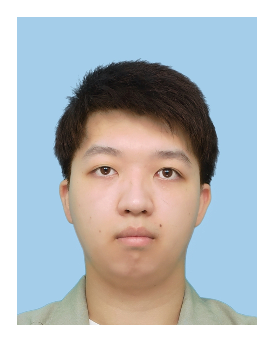
\includegraphics[width=\linewidth]{product.eps}
\end{minipage}
\hfill
\begin{minipage}[H]{0.75\textwidth}
  \raggedleft
  {\LARGE\bfseries 根岸 颯}\\[3mm]
  {\large 原子核物理学研究}\\[2mm]
  {\normalsize 千葉大学融合理工学府 修士課程在学中}\\[3mm]
  \begin{tabular}{ll}
    \textcolor{black}{Email:} & \texttt{25wm2106@student.gs.chiba-u.jp}\\
    \textcolor{black}{GitHub:} & \href{https://github.com/Negsn0}{\textcolor{black}{https://github.com/Negsn0}}\\
    \textcolor{black}{電話番号:} & 080-6686-2237
  \end{tabular}
\end{minipage}

\vspace{8mm}

% プロフィール
\section*{プロフィール}
\begin{tcolorbox}[
  colback=lightgray,
  colframe=primary,
  boxrule=1pt,
  arc=3pt,
  left=8pt,
  right=8pt,
  top=8pt,
  bottom=8pt
]
原子核物理学の研究を通じて、\highlight{課題発見能力}と\highlight{観察力}を磨いてきました。人と協力しながら新しいことに挑戦することが好きで、理想と現実のギャップを埋める努力にやりがいを感じています。

高校時代には体育祭の実行委員として競技内容を改革し、後輩への引き継ぎ資料も整備。現在の研究でも数値計算のエラーを特定・解決し、問題解決力を発揮しています。
\end{tcolorbox}

\vspace{6mm}

% 学歴
\section*{学歴}
\begin{itemize}[leftmargin=12mm, itemsep=3mm]
  \item \textbf{千葉大学 融合理工学府 修士課程} \textcolor{secondary}{在学中(2025年4月~)}
  \item \textbf{千葉大学 理学部物理学科} \textcolor{secondary}{卒業(2021年4月~2025年3月)}
  \item \textbf{安田学園高等部 S特コース} \textcolor{secondary}{卒業(2018年4月~2021年3月)}
\end{itemize}

\vspace{6mm}

% 研究内容
\section*{研究内容}
\begin{itemize}[leftmargin=12mm, itemsep=4mm]
  \item \highlight{専攻分野}:原子核物理学(数値計算による物理現象の解明)
  \item \highlight{卒業研究}:有限温度における原子核の相転移現象の数値解析
  \begin{itemize}[leftmargin=8mm, itemsep=2mm]
    \item C言語・JuliaによるBCS状態の相転移追跡システム構築
    \item AI技術を活用した並列化処理により計算効率向上
  \end{itemize}
  \item \highlight{修士研究}(進行中):角運動量射影による対称性の回復手法開発
  \begin{itemize}[leftmargin=8mm, itemsep=2mm]
    \item Fortranコードの最適化とJuliaへの移植
  \end{itemize}
\end{itemize}

\vspace{6mm}

% 技術スキル
\section*{技術スキル}
\skillbox{
\begin{itemize}[leftmargin=8mm, itemsep=3mm]
  \item \highlight{プログラミング言語}:Python, Julia, Fortran, C言語
  \item \highlight{開発環境・ツール}:Git, GitHub, VSCode, Linux(Ubuntu)
  \item \highlight{専門分野}:数値計算, 並列化処理, 物理シミュレーション
\end{itemize}
}

\vspace{6mm}

% 資格
\section*{保持資格}
\begin{itemize}[leftmargin=12mm, itemsep=3mm]
  \item \textbf{TOEIC 760点} \textcolor{secondary}{(2024年取得)}
  \item \textbf{基本情報技術者試験 合格} \textcolor{secondary}{(2024年取得)}
  \item \textbf{普通自動車免許} \textcolor{secondary}{(2022年取得)}
\end{itemize}

\vspace{6mm}

% 職歴・アルバイト
\section*{職歴・アルバイト経験}
\begin{itemize}[leftmargin=12mm, itemsep=4mm]
  \item \highlight{東京個別指導学院} \textcolor{secondary}{(2021年~)}
  \begin{itemize}[leftmargin=8mm, itemsep=2mm]
    \item 塾講師、リーダー業務
    \item 生徒のやる気を引き出す指導とチーム運営(2022・2024年)
  \end{itemize}
  \item \highlight{安田学園中高} \textcolor{secondary}{(2021年~2023年)}
  \begin{itemize}[leftmargin=8mm, itemsep=2mm]
    \item 学習チューターとして個別最適化指導を実施
  \end{itemize}
\end{itemize}

\vspace{6mm}

% プロジェクト実績
\section*{研究・開発プロジェクト}
\begin{itemize}[leftmargin=12mm, itemsep=4mm]
  \item \highlight{原子核物理シミュレーション開発}
  \begin{itemize}[leftmargin=8mm, itemsep=2mm]
    \item BCS理論・HFB法による高精度な数値計算システムの構築
  \end{itemize}
  \item \highlight{AI活用による科学計算の最適化}
  \begin{itemize}[leftmargin=8mm, itemsep=2mm]
    \item \textbf{ChatGPT}や\textbf{Cursor}を活用した並列計算で計算時間を短縮
  \end{itemize}
  \item \highlight{レガシーコードの現代化}
  \begin{itemize}[leftmargin=8mm, itemsep=2mm]
    \item Fortran→Julia移植による保守性と開発速度の改善
  \end{itemize}
\end{itemize}

\end{document}